% This is a sample LaTeX input file.  (Version of 12 August 2004.)
%
% A '%' character causes TeX to ignore all remaining text on the line,
% and is used for comments like this one.

\documentclass{article}      % Specifies the document class

\usepackage{graphicx}		 % Need this to include images
\graphicspath{{images/}}

\usepackage[]{todonotes}
\usepackage{fancyvrb}

\usepackage{hyperref}
\usepackage{xcolor}
\hypersetup{
    colorlinks,
    linkcolor={black!50!black},
    citecolor={black!50!black},
    urlcolor={black!80!black}
}

\usepackage[acronym, nomain, style=tree, toc, section=section, nogroupskip=true]{glossaries}
%% load and typeset glossaries
\makeglossaries
\loadglsentries{acronyms.tex}
\glsenablehyper

\usepackage{listings}
\usepackage{subcaption}
\usepackage{titlesec}
\newcommand{\sectionbreak}{\clearpage}
%% Define a HUGE 
\makeatletter
\newcommand\HUGE{\@setfontsize\Huge{50}{60}}
\makeatother

\begin{document}             % End of preamble and beginning of text.

%%%%%%%%%%%%%%%%%%%%%%%%%%%%%%%%%%%%%%%%%%%%
%%%%%%%%%%%%%%%%%%%%%%%%%%%%%%%%%%%%%%%%%%%%
%titlepage
\thispagestyle{empty}
\begin{center}
\begin{minipage}{0.9\linewidth}
\flushright
	      		 
	%University logo
    
\includegraphics[width=0.5\linewidth]{univie.jpg}\par
    \vspace{1.5cm}
\centering 	
    % Title
	{\scshape{\HUGE Bachelorarbeit\par}}
	\vspace{1cm}
	%Thesis title
    {\scshape{\Large An IoT based Monitoring System using Raspberry Pis and Seattle Testbed\par}}
    \vspace{2cm}
    
  
 verfasst von \linebreak 
 {\Large Peter~Klosowski\par}
 	\vspace{1.3cm}
angestrebter akademischer Grad \linebreak
 {\Large Bachelor of Science (BSc)\par}
	\vspace{1.3cm}

\flushleft
	

\begin{tabular}{ll}
Wien, 2018	\linebreak
\vspace{1cm}&   \\
  Studienkennzahl lt. Studienblatt: & A 033 521 \vspace{0.3cm} \\ 
  Fachrichtung: & Informatik -  Medieninformatik \vspace{0.3cm} \\
  Betreuer: & Univ.-Prof.~Dipl.-Math.~Peter~Reichl,~M.A.~St. \\
  Gutachter: & Dr.~Albert~Rafetseder,~BSc~MSc \vspace{0.3cm} \\
 \end{tabular}
    
\end{minipage}
\end{center}
\clearpage

\pagebreak

%%%%%%%%%%%%%%%%%%%%%%%%%%%%%%%%%%%%%%%%%%%%
%%%%%%%%%%%%%%%%%%%%%%%%%%%%%%%%%%%%%%%%%%%%
\thispagestyle{empty}
    Ich versichere an Eides statt durch meine Unterschrift, dass ich die vorstehende Arbeit selbst\"andig und ohne fremde Hilfe angefertigt und alle Stellen, die ich w\"ortlich oder ann\"ahernd  w\"ortlich  aus  Ver\"offentlichungen  entnommen  habe,  als  solche  kenntlich  gemacht  habe,  mich  auch  keiner  anderen  als  der  angegebenen  Literatur  oder  sonstiger Hilfsmittel bedient habe. Die Arbeit hat in dieser oder \"ahnlicher Form noch keiner anderen Pr\"ufungsbeh\"orde vorgelegen.

    \vspace{1.5cm}

    \noindent\makebox[2.5in]{\hrulefill}\\
    \small Peter Klosowski, Wien, 28. Februar 2018

\newpage


\pagenumbering{Roman}

%%%%%%%%%%%%%%%%%%%%%%%%%%%%%%%%%%%%%%%%%%%%%%%%%%%%%%%%%%%%%%%%%%%%%%%%%%%%%%%%
\section*{Acknowledgements}
\addcontentsline{toc}{section}{Acknowledgements}%

First and foremost, the author wants to thank his supervisor, Peter Reichl. Not only is his first name a great one, but his support throughout this semester was extremely well received and welcomed. His feedback and advice improved this work immensely.
\\[1em]

Special thanks go to the author's bachelor advisor, Albert Rafetseder, for the hours spent together reviewing, discussing, and writing the numerous emails that were exchanged over the past five months. His patience with the author and qualified input was most appreciated.
\\[1em]

The author would also like to thank his friends and family. The help was highly valued, for standing by the authors side, proof reading this work and also distracting the author countless of times.
\\[1em]

Furthermore, the author wants to thank STMicroelectronics for providing free samples of their temperature, humidity, and pressure sensors to support this bachelor thesis.

%%%%%%%%%%%%%%%%%%%%%%%%%%%%%%%%%%%%%%%%%%%%%%%%%%%%%%%%%%%%%%%%%%%%%%%%%%%%%%%%
\section*{Abstract}
%\phantomsection
\addcontentsline{toc}{section}{Abstract}%

Single board computers, such as the Raspberry Pi have been popular for years. More and more, \gls{IoT} devices are pushed onto the market to satisfy customer needs. This bachelor thesis proposes an approach to build a decentralized environmental monitoring system that is flexible regarding sensor compatibility. The system developed in this thesis uses Seattle Testbed as a code base and as a result authorized users were able to collect data via the Internet. The \gls{Repy} \gls{API} was extended with compatible drivers for the sensors. To visualize the data, a website was developed using Angular-nvD3, that is based on the modern plotting tool D3. 

\newpage

\phantomsection
% Set to either section or chapter depending on chosen template
\tableofcontents		% Table of Contents
\newpage

\makeatletter
\begingroup
\let\clearpage\relax
\let\cleardoublepage\relax
\phantomsection
\addcontentsline{toc}{section}{Figures}%
\section*{Figures}
\@starttoc{lof}%
\bigskip
\phantomsection
\addcontentsline{toc}{section}{Tables}%
\section*{Tables}
\@starttoc{lot}
\endgroup
\makeatother

\glsaddall
\begingroup % printglossar{y,ies} forces a cleardoublepage between glossaries and after it, we supress this here
	\let\clearpage\relax
	\printglossaries
\endgroup


%%%%%%%%%%%%%%%%%%%%%%%%%%%%%%%%%%%%%%%%%%%%%%%%%%%%%%%%%%%%%%%%%%%%%%%%%%%%%%%%
% Reset the page counter for the actual content
\cleardoublepage
\pagenumbering{arabic}
\setcounter{page}{1}


%%%%%%%%%%%%%%%%%%%%%%%%%%%%%%%%%%%%%%%%%%%%%%%%%%%%%%%%%%%%%%%%%%%%%%%%%%%%%%%%
\section{Motivation and Theoretical Background}

Since the release of the Raspberry Pi \cite{raspberry}, a low-cost single-board computer, a groups of hobbyists, academics, companies, hackers and \acrshort{IT} criminals, have grabbed onto this trend of \acrfull{IoT} and are experimenting. They have built useful and unique devices with it, such as smart locks and mirrors. One field widely explored is the monitoring of various environments. Using sensors to expand the application of the Raspberry Pi, it is possible to cover a lot of different use cases, e. g. connecting a camera to observe the surroundings or record climate change over time. Flexibility regarding the operating system, programming language, sensors and expanding the Raspberry Pi with shields are just a few of the advantages, when working with the Raspberry Pi \cite{rasberry}. 

This kind of embedded systems are all part of \gls{IoT}. \gls{IoT} is a term for every object that gets hooked up to the Internet through devices such as the Raspberry Pi. The goal of embedded system is to make human lives easier and improve the live quality. This is achieved by offering new functions to older devices and even control them when nobody is near them. On the other hand, they need to be developed with security in mind to prevent attackers getting access to them. \cite{iot}

The sensors used for this project were collecting various kinds of data. One of them was a light sensor. It recorded visible and \gls{IR} light. Visible light has a wavelength of 400 to 770 \gls{nm} and, as the name states, it is visible to humans. Light with a  wavelength from 1 to 400 \gls{nm} is called \gls{UV}. This light hurts the human skin and might cause skin cancer in the worst case scenario. The light closest to the visible red light is called \gls{IR} light. It can go up to 1 \gls{mm}, starting at a wavelength of 760 \gls{nm}, and the human perceives it as heat. \cite{lightDesc}

Another sensor was responsible to collect data regarding air quality. \Gls{TVOC} are polluting the air. The higher the concentration of these compounds is, the more harmful it is to humans. Without airing a room regularly, the health of humans and animals inside there is at risk. Electronic devices such as printers and \glspl{PC} are emitting the substances ozone and benzene, that are included in \glsdisp{VOC}{VOCs}. \Gls{CO2} is part of \glspl{VOC} as well and therefore, humans are contributing to that by breathing.
\cite{airQualitySensor}

The sensors can be connected to a Raspberry Pi through the \gls{GPIO} pins. Some of them are capable of utilizing the \gls{I2C} protocol that allows multiple connections of peripherals. Newer versions of the Raspberry Pi, starting with Revision B, are using bus 1 and the \gls{GPIO} pins 3 (\gls{SDA}) and 5 (\gls{SCL}) to exchange messages with the sensors. The bus is a system that allows communication between two components and the pins are the physical interface. Each connected slave has its own address that is up to 7 bits long. It is worth mentioning that two slaves cannot have the same address because it would conflict with messaging the right receiver. \cite[p.~167ff]{masteringPi}

In this work, a Raspberry Pi 2B was combined with three different sensors. Knowing that the finished box would be used by other academics and students for their projects it was necessary to meet some requirements. Ideally, the box should not be too expensive so multiple ones can be produced and set up. To do efficient experiments, a decentralized approach was essential to deploy them for different scenarios and use cases. Therefore the execution of specific software code on multiple boxes to collect data was necessary. Depending on what kind of data should be collected, different code snippets would be used and uploaded to the boxes. They should be in sync even if the units do not know of each other. Another point was to build a \gls{FLOSS}, so it should be accessible in the future, and can be used to enrich their projects. Open Data was an important aspect as well. For example, if desired, it should be possible to upload all collected data and present it to readers who observe the development of it and the project. This way, it is possible to provide more transparency, contribute to the public and provide a platform to reuse collected data \cite{openData}.

To solve problems with cluster management, software updates or code pushing a software solution was used, called Seattle. Seattle is described as ``a free, open-source platform for networking and distributed systems research" \cite{seattleGithub}. Seattle runs on many devices allowing researchers and students to access machines that are connected to the network through the Internet. They are limited though, and are just allowed to work inside a \gls{SB} that limits the use of \gls{CPU} power, memory and storage space. \cite{seattleFence} \cite{seattleSandbox}


\subsection{Application of the Box}

As previously mentioned, the expected field of use is more academic, but that does not imply the practical use. It was already clear in the beginning, that a more general approach should be taken. Therefore, a quick replacement of one or more sensors would be necessary at some point. 

A possible application would be to use moisture, temperature, light and water quality sensors, pair them with the Raspberry Pis. After that, deploy all of it with the software build to measure the soil in a garden or perhaps even a park or golf course. In an apartment it would be possible to use this kind of technology to improve the health of home plants.

Another good use would be to monitor the well being of occupants in an apartment by installing air quality, temperature, humidity, and pressure sensors. If one of those values would indicate a bad influence to the health or comfort of the home owner, then it would be a good idea to take countermeasures. This could also safe lives, if the occupant gets notified in time to leave the premises.

\subsection{Overview of this work}

This document is structured as followed. The previous introduction gave a small overview over the motivation and theoretical background of this work. Important terms were defined and described. Section \ref{sec:relatedWork} compares this work with other related work and points out the difference to previously published papers. An overview of the system design is given in Section \ref{sec:systemDesign}. The use case and deployment diagram are described in detail. The implementation of drivers, the process of extending the Seattle \gls{SB}, the website for visualization, and wiring the sensor components to the Raspberry Pi are part of Section \ref{sec:implementation}. In Section \ref{sec:evaluation}, the results of a functional and experiment evaluation are described. The last part of this work, Section \ref{sec:conclusio}, is the conclusion. It elaborates on positive outcomes, issues, that appeared during development, and future work.

%%%%%%%%%%%%%%%%%%%%%%%%%%%%%%%%%%%%%%%%%%%%%%%%%%%%%%%%%%%%%%%%%%%%%%%%%%%%%%%%
\section{Related Work} \label{sec:relatedWork}

Several \gls{IoT} solutions were thought of and developed in the past.  Many of these following papers describe use cases of decentralized \gls{IoT} devices utilizing different technologies. 

Reinfurt L. et al \cite{iotPatterns} gathered five different state-of-the-art design patterns regarding \gls{IoT} that have been identified by reviewing existing products. They recognized the problems that occurred during the software implementations of \gls{IoT} devices and also offered a satisfying solution. 

Shete R. and Agrawal S. \cite{urbanRasp} presented a low cost urban climate monitoring system using a Raspberry Pi and various sensors such as air quality, light and temperature. The collected data was uploaded to Adafruit IO, a cloud \gls{IoT} system, via Wi-Fi. Through the use of an \gls{MQTT} broker, the data was distributed to subscribed user.

Roselle B. Anire et al \cite{raspNet} focused on monitoring soil in a greenhouse. A \gls{WSN} combined with the ZigBee protocol was used as a solution. Four Raspberry Pis were deployed and connected together over the network and data was sent to a PC that aggregated it. A simple \gls{GUI} was created to visualize this data and inform the farmer about the soil conditions.

Ibrahim M. et al \cite{smartEnv} collected environmental data using a Raspberry Pi and sensors connected to it, including a sensor registering earthquakes was installed. A protocol, \gls{EEML}, was used to share the sensor data with another remote device such as a laptop, smartphone or a web service in the cloud. 

Wixted A. et al \cite{loraEval} presented LoRa and the LoRaWAN protocol and compared it to other state-of-the-art technologies that are used for \gls{IoT}. The protocol is explained and evaluated on reliability and performance with a positive outcome, such as network coverage in hard-to-reach places with numerous gateways. 

Related to this work, \cite{urbanRasp}, \cite{raspNet}, and \cite{smartEnv} are also building \gls{IoT} systems. They are deployed in different environments. Taking \cite{urbanRasp} as a model, the low cost approach of the climate monitoring system affected the sensor components that were bought for this project. Sensors for air quality, light and temperature were used. For future work it would be possible to update the visualization website using \gls{MQTT} and implement LoRaWAN, that was used in \cite{loraEval}. To build a secure and reliable \gls{IoT} environment, it is advised by \cite{iotPatterns} to make use of the \gls{IoT} patterns discussed in that paper. Seattle uses some of this patterns that improve the \gls{IoT} device.

%%%%%%%%%%%%%%%%%%%%%%%%%%%%%%%%%%%%%%%%%%%%%%%%%%%%%%%%%%%%%%%%%%%%%%%%%%%%%%%%
\section{System Design and Solution Concept} \label{sec:systemDesign}

Based on the requirements discussed in the introduction of this work, a software design was developed. The whole documentation, partially described here, can also be retrieved from the personal GitHub repository\footnote{ \url{https://github.com/Peter0014/COSY-Lab-IoT-Box/tree/master/DesignDoc}}. Regarding the following content, it is worth mentioning that the existing Seattle Testbed \cite{seattleHomepage} was used as a codebase. This decision affected some of the software design as a result, such as the deployment and the use cases.

All of the following system designs were modeled with the \gls{UML} standard \cite{uml}. That standard is widely used in software engineering and allows a quick understanding of high and low level architectures with the provided tools. It is also capable of creating business and similar models, but these were not necessary this time, because this work was a pure software solution.

\subsection{System Overview -- Use Case}

At the beginning of the project, the future features were defined using a Use Case diagram. Figure \ref{fig:useCase} illustrates six use cases that were actually implemented. There are two actors that will be using them. In this case the ``User" will be any person who has access to the system and is allowed to operate with it. The ``\gls{IoT} box" is the combination of a Raspberry Pi, sensors and the Seattle software build. The use cases described in the following Sections \ref{sec:seattleStart} to \ref{sec:seattleEnd} are handled by Seattle. Use cases discussed in Sections \ref{sec:contrStart} to \ref{sec:contrEnd} are contributions of this thesis.

\begin{figure}[ht]
	\makebox[\textwidth][c]{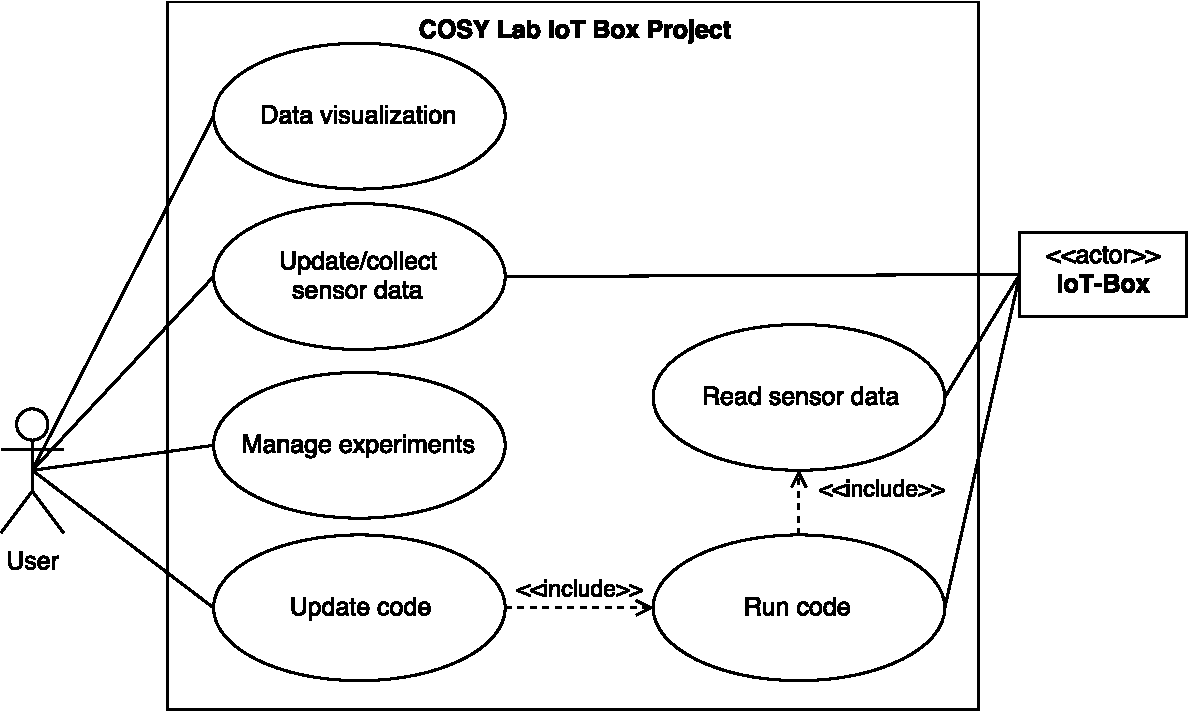
\includegraphics[width=13.5cm]{Use_Case_Diagram.pdf}}
	\caption{Use case diagram describing the \gls{CoSy} Lab \gls{IoT} box Project}
	\label{fig:useCase}
\end{figure}

\subsubsection{Manage Experiments} \label{sec:seattleStart}

The use case includes two work flows regarding experiments that are run on one or more \gls{IoT} boxes. Experiments in this scope are installations of the software on the Raspberry Pis. It is possible to register new experiments and remove ones that are no longer needed. Also, secure access should be guaranteed in case a user who is not authorized tries to access this information.

\subsubsection{Update Code}

To adapt to different use cases of the boxes, it is necessary to update its purpose and code over the Internet. The user is able to upload a code snippet with the functions that he or she wants to run and decides to push it to one or more boxes. Here the user has the choice which sensor data is collected, the interval, and the file format it is saved in. After a successful upload, the boxes will try to run it and begin its data collection or return an error to the user. Access control should also be implemented in this case to allow only authorized users to update code fragments.

\subsubsection{Run Code} \label{sec:seattleEnd}

All uploaded codes needs to be run by the boxes. It is important to do so the user is able to collect data from the sensors attached to the box. Depending on the code that is pushed, different types of sensor data can be fetched and saved.

\subsubsection{Read Sensor Data} \label{sec:contrStart}

First, the data needs to be collected. Over the \gls{I2C} bus a connection will be established and sensor data will be fetched with help of the drivers imported into the Seattle \gls{SB} beforehand. The uploaded code decides which sensors are contacted and the time interval in which new data is appended to a file. Depending on the use case, it should be possible to use different sensors that were originally not thought of at the beginning of this work or are good additions to the existing ones. Because every sensor is different, like newer revisions or different kinds of design and companies, it will be necessary to update the software loaded onto the Raspberry Pis. This process is explained in more detail in Section \ref{sec:implementation}.

\subsubsection{Collect Sensor Data}

It is possible to download the files over the Internet produced by the user supplied code and after some sensor data was read and saved to the boxes. The data can be used to plot some graphs using the dedicated website that was developed during this work and is described further in Section \ref{sec:implementation} and the next use case. Regarding the Open Data requirement, it is possible to publish that data for everybody to download, use, share, and work with.

\subsubsection{Data Visualization} \label{sec:contrEnd}

  The data visualization is another crucial part of this work. It would also be possible to visualize the data with applications such as Microsoft Excel\footnote{\url{https://products.office.com/de-at/excel}} and similar tools. The end user would download raw data sets to import them into those tools to plot charts. On the other hand it is useful to offer the user a tool, or web page in this case, where he or she can upload data and it is automatically visualized. Additionally, it would be possible to store data on the web server to demonstrate it using the plotting tool that is specifically customized for the format and output of the boxes. 

\subsubsection{Alternatives}

Searching for solutions, it was decided that Seattle was a satisfying approach in this case. However, there were other thoughts and alternatives before Seattle came up. For example, it was an option to built a decentralized system behind it from scratch. \gls{IoT} patterns mentioned in \cite{iotPatterns} would have been used. Device shadowing for a persistent storage of the data allow to reach a device, even if it is offline and unavailable right now. Implementing a rules engine would have supported with dynamic routines for fetching sensor data if the user sent a particular message to the system. If the boxes were used in outdoor places that are not overlooked or unsecured, it would also have been helpful to have a remote lock feature.

Some of these patterns are available in the Seattle software, such as a rules engine that supports actions via a special scripting language. Additionally, it also covers and solves problems such as cluster management and code pushing. It was also decided with the supervisor that building an \gls{IoT} system from scratch would be too large a scope for a bachelor project.

\subsection{System Overview -- Software Deployment}

The software deployment illustrates the distribution of software artifacts. Looking at Figure \ref{fig:deployment} one can 
differentiate between four different devices: 
\\
\begin{description}
	\item[``User Client"]
	is typically the home computer of the end user
	\item[``Web Server"]
	is used for the visualization of the data
	\item[``Raspberry Pi"]
	is part of the subsystem ``\gls{IoT} box" and executes the user provided code 
	\item[``Various Sensors"]
	are part of the subsystem ``\gls{IoT} box" and collect data from the environment
\end{description}

\noindent
\\The components are described in more detail in the following sections.

\begin{figure}[ht]
	\makebox[\textwidth][c]{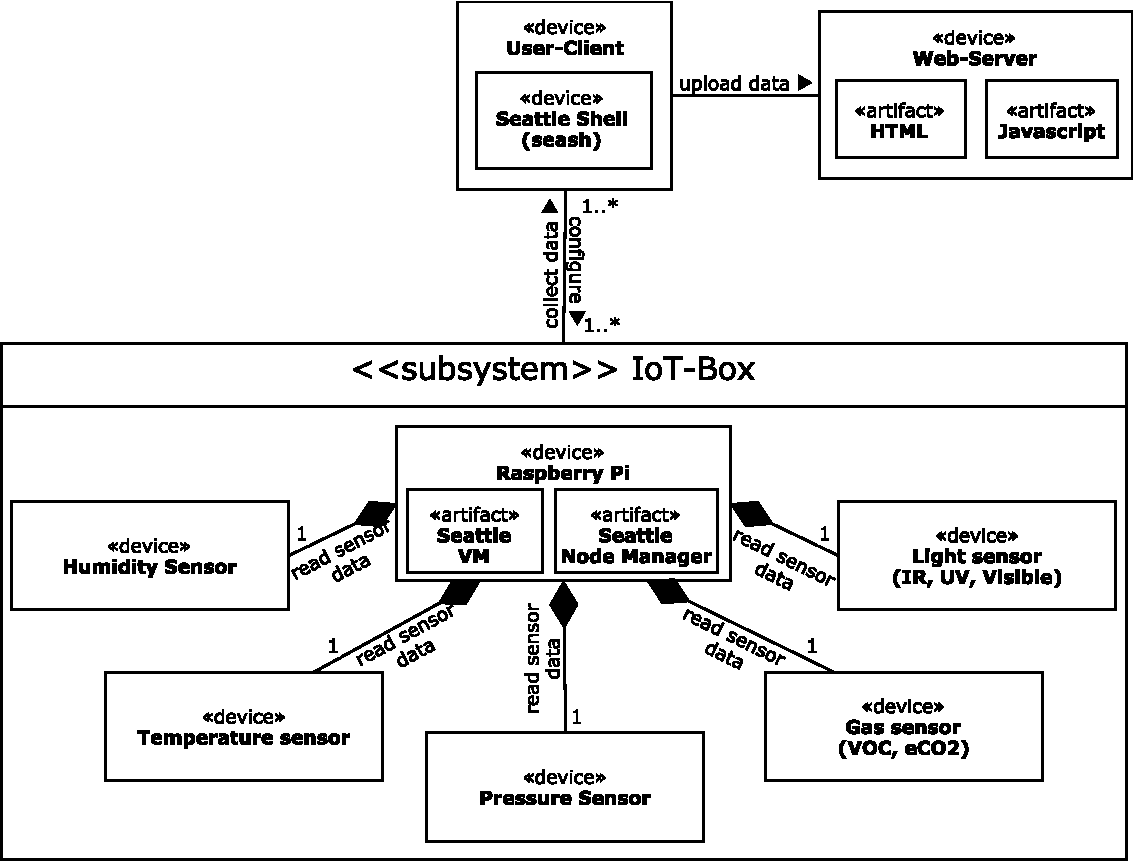
\includegraphics[width=13.5cm]{Deployment_diagram.pdf}}
	\caption{Deployment diagram}
	\label{fig:deployment}
\end{figure}

\subsubsection{Raspberrry Pi}

The hardware runs the Seattle software. The Seattle \gls{VM} executes the user provided code and prevents malicious content that could potentially break out of the \gls{VM} to get access to the system it is running on. It also prevents the application from using too many resources from components such as the \gls{CPU} or memory. \cite[p. 38]{seattlePaper} \cite{seattleFence}

The Seattle Node Manager is important for several reasons. First, it manages access control and allows just authorized parties to execute code on the device it is installed on. At the same time, it provides an interface to upload code, manage a \gls{VM}, and download collected data and logs from it. \cite[p. 38]{seattlePaper}

Different sensors connected to a Raspberry Pi are components of the subsystem ``\gls{IoT} box". In this case, the sensors are: a humidity, temperature and pressure sensor, a gas sensor collecting \gls{TVOC} and \gls{eCO2} data, as well as a light sensor for \gls{IR}, \gls{UV} and visible light. All of them are described in more detail in Section \ref{sensorDesc}. Using Seattle allows to have one or many \gls{IoT} boxes that are configured by one or many authorized user clients.

\subsubsection{Web Server}

The visualization of the data takes place on the web server, or to be precise, on the user client by processing the JavaScript files that are provided by the server. It is possible to load a file with the sensor data into the script and let it plot different graphs for every available data entry. The output is presented to the user through the web page in his or her browser. Regarding Open Data, it is also possible to save files on the web server by the administrator to share it with the public.

\subsubsection{User-Client}

Through \gls{seash}, it is possible to connect to Raspberry Pis if the user is authorized to do so. The user is able to install \gls{seash} onto his or her device and configure the \gls{VM}, push code to it, as well as to collect the data that is generated through his or her code. \Gls{seash} operates here as a service manager and allows the interaction with the node manager \cite[p. 38]{seattlePaper}. The user client also connects to the web server via a browser of his or her choice and opens up the web page to process his data, that he downloaded from the Raspberry Pis.

%%%%%%%%%%%%%%%%%%%%%%%%%%%%%%%%%%%%%%%%%%%%%%%%%%%%%%%%%%%%%%%%%%%%%%%%%%%%%%%%
\section{Implementation} \label{sec:implementation}

There are three parts to the implementation. The first part was the decision of buying several sensors, built a hardware interface, connect them to the Raspberry Pi and test them. The second part consisted of developing the software to operate the sensors and extend Seattle in that way, that it can call those software functions. In the last part, a website was built that can be used for visualization and informing other people about the project and progress.

\subsection{Exploring Sensors} \label{sensorDesc}

Looking for different use cases that were not just practical but also useful in the sense of doing research with them, the decision was made to buy three different sensors. The sensors measure 7 different physical quantities. In combination, they were collecting useful data about the environment that could be used in all rooms of a home, in a lab, and outdoors. Furthermore, all sensors are breakout boards by the company Adafruit\footnote{\url{https://www.adafruit.com/}}. It was necessary to solder the header onto the \gls{PCB} and was also required that all sensors support the \gls{I2C} protocol.

\subsubsection{Temperature, Barometric Pressure and Humidity Sensor} 

One sensor is a BME280 environmental sensor was manufactured by Bosch\footnote{\url{https://www.bosch-sensortec.com/}}. It measures temperature, humidity and barometic pressure, also known as atmospheric pressure. It has an accuracy of $\pm$ 3\% regarding humidity, $\pm$ 1 \gls{hPa} with barometic pressure and $\pm$ 1.0°\gls{C} with temperature. \cite{bme280}

Additionally, STMicroelectronics\footnote{\url{http://www.st.com/}} provided sample sensors from their product line. For one, the HTS221 for relative humidity and temperature and the LPS25HB for absolute pressure was sent to support the project. They have an accuracy of $\pm$ 0.5°\gls{C} regarding temperature between 15°\gls{C} and 40°\gls{C}, $\pm$ 3.5\% with humidity and $\pm$ 1 hPa  with barometic pressure. \cite{stHum} \cite{stPress}

\subsubsection{Light Sensor} 

The SI1145 light sensor from SiLabs\footnote{\url{https://www.silabs.com/}} calculates the \gls{UV} index based on the \gls{IR} and visible light from the sun. As a side note, this sensor measures light levels and the \gls{IR} and visible light values are ``based on how much light the sensor sees, and there's no `units' to them". \cite{si1145}

\subsubsection{Air Quality Sensor} \label{sec:airQual}

There is a lot of air pollution in big cities that is harmful to every person if it is present in high amounts. This is especially prominent in the morning when people drive to work. The \gls{CO2} pollution is increasing immensely \cite{carWork}. To measure that, it was decided to install an air quality sensor - the CCS811. The chip was developed by ams\footnote{\url{http://ams.com/}} and collects \acrfull{eCO2} and \acrfull{TVOC} data. It has a range from  400 to 8192 \gls{ppm} regarding \gls{eCO2} and 0 to 1187 \gls{ppb} with \gls{TVOC}. The value \gls{eCO2} is also a bit misleading because it is based on the measured \gls{TVOC}. An increasing in \gls{TVOC} indoors also quite often means an increase in \gls{CO2}, because a person entered the room. This sensor does not measure the amount of \gls{CO2} in the air.

It is also recommended to run it 48 hours after buying it to burn it in. Before starting to read data, it is always necessary to let the sensor run for 20 minutes. Unfortunately, after starting the data collection for the evaluation it was clear that the air quality sensor does not work properly with the Raspberry Pi because the sensor uses clock stretching that the Pi does not support. The sensor will be replaced in the future. \cite{ccs811}

\subsection{Wiring}

The Fritzing\footnote{\url{http://fritzing.org}} application was used to visualize the wiring of the sensors with the Raspberry Pi. Figure \ref{fig:wiring} illustrates all three previously mentioned sensors on a breadboard to the left of a Raspberry Pi 2B. A breadboard is perfect for testing purposes because it does not require any soldering of components.

\begin{figure}[ht]
	\makebox[\textwidth][c]{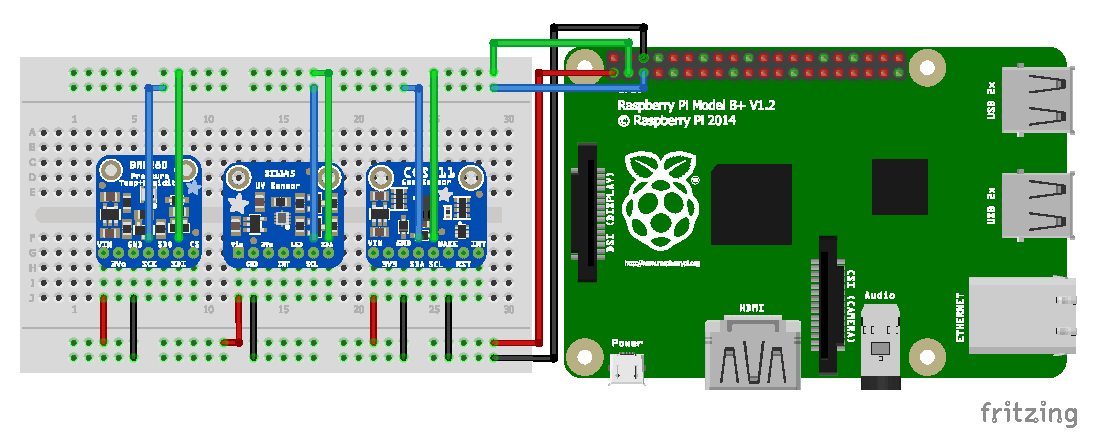
\includegraphics[width=13.5cm]{Sketch_Breadboard.pdf}}
	\caption{Wiring diagram of an \gls{IoT} box}
	\label{fig:wiring}
\end{figure}

Two wires are necessary to connect the sensors to the physical interface of the \gls{I2C} bus. The blue wire represents the connection to pin 5, the \gls{SDA} pin. Pin 3, or \gls{SCL}, connects to the sensors through the green wire. It is also necessary to power the sensors. Therefore, the red wire is attached to the 3.3 \gls{V} pin and the black one to the ground.

The wires were connected, according to the \gls{I2C} wiring on the websites from Adafruit. From left to right, the sensors in Figure \ref{fig:wiring} are the BME280, the SI1445, and the CCS811. Every sensor receives power at the pinout with the label \texttt{Vin}. The ground is at \texttt{GND}. The \gls{SDA} and \gls{SCL} pinouts are labeled \texttt{SDA} and \texttt{SCL}. The CCS811 needs another ground wire that connects to the \texttt{WAKE} pinout. \cite{bme280} \cite{ccs811} \cite{si1145}

\subsection{Software Development}

The next step taken after connecting the sensors to the Raspberry Pi over the \gls{I2C} dedicated Pins was to develop software classes and extend the Seattle \gls{Repy} V2 code to call the functions in these classes. Figure \ref{fig:classDiagram} shows a small excerpt of these classes that are described in the following sections.

\begin{figure}[ht]
	\makebox[\textwidth][c]{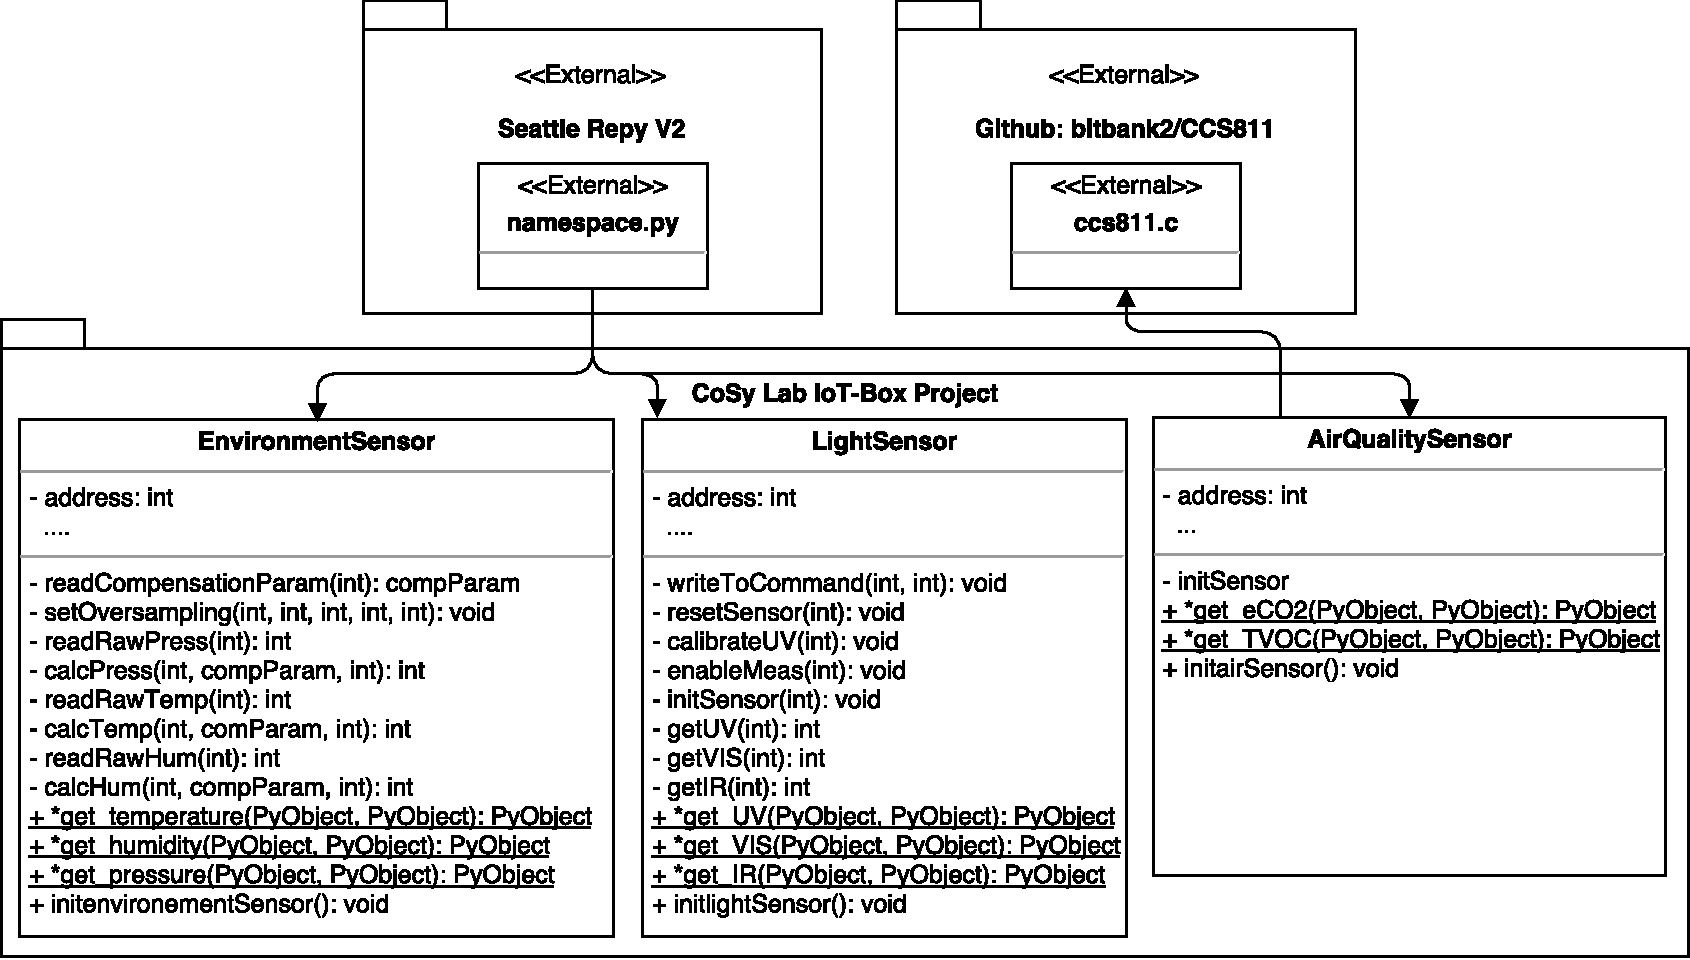
\includegraphics[width=13.5cm]{Class_Diagram_Cropped.pdf}}
	\caption{Excerpt of the class diagram}
	\label{fig:classDiagram}
\end{figure}

\subsubsection{Writing the Classes}

Seattle is programmed using the Python language. Therefore, Python would have been a good choice for this situation. Consequently, it was inevitable to use a wrapper if C code would be used to extend the existing Seattle code base. 

The decision was made based on a personal preference. Being more in contact C through internships and courses at the university, it was easier to perform this project with the already available know-how. Looking for available resources online, there was an official section in the documentation of Python about extending it with C\footnote{\url{https://docs.python.org/2/extending/extending.html}}, as well.

With the CPython \gls{API}, it is possible to use C code in a Python class. It is imported like any other module in Python. However, the C class needs to be prepared before Python is able to call it. A method is necessary for Python to initialize the methods used in the C code. Python also cannot process the data types used in C. Therefore, the data type \texttt{PyObject} needs to be created and returned.

The classes \texttt{EnvironmentSensor}, \texttt{LightSensor} and \texttt{AirQualitySensor} are drivers, which read various values from the sensors. They are imported by Seattle \gls{Repy} V2 in the \texttt{namespace.py} class. To compare development time, the class fetching the air quality values is just a wrapper and uses the implementation from Github by the user bitbank2\footnote{\url{https://github.com/bitbank2/CCS811}}. Writing just a wrapper for an existing driver took two hours. Depending on the complexity of a sensor, it could take effort and time to implement a driver. The drivers for the BME280 and SI1145 took each three to four days to implement.

\subsubsection{Extending Seattle with C}

To extend the Seattle \gls{SB} with sensor functions, drivers were written with the help of the documentations from the sensors. After testing them on the device itself and checking that the right values were returned, a shared library and Python module was created using the \gls{GCC}. For example, a shell command could be written as in Figure \ref{fig:buildCommand}.

\begin{figure}[ht]
	\centering
	\begin{BVerbatim}
gcc -shared -Xlinker -export-dynamic -o environmentSensor.so 
-I/usr/include/python2.7/ -lpython2.7 -lwiringPi 
BME280_TempSensor.c
	\end{BVerbatim}
	\caption{Build command for a shared library}
    \label{fig:buildCommand}
\end{figure}

In this case a shared library is created with the parameters \texttt{-shared -Xlinker \mbox{-export-dynamic}}. The output file would be \texttt{environmentSensor.so} and the input file is the C class \texttt{BME280\_TempSensor.c}. The WiringPi and Python libraries and imports are necessary to build the class properly.
The \texttt{.so} file, that is produced calling that command, can be loaded into Python as a module now. Visible are just special functions though. Looking at Figure \ref{fig:classDiagram}, the static functions that return the \texttt{PyObject} are added in the init function (like \texttt{initenvironmentSensor()}) so that Python is able to work with them.

\begin{figure}[ht]
	\centering
	\begin{BVerbatim}

...
import environmentSensor
...
RPI_ENVIRONMENT_SENSORDATA_WRAPPER_INFO = {
    'get_temperature' :
        {'func' : environmentSensor.get_temperature,
         'args' : [],
         'return' : Float()},
         ...
}
USERCONTEXT_WRAPPER_INFO.update
	(RPI_ENVIRONMENT_SENSORDATA_WRAPPER_INFO)
	\end{BVerbatim}
	\caption{Import of the shared library environmentSensor.so in namespace.py}
    \label{fig:pythonLibrary}
\end{figure}

Having a working Python module available, it was now possible to extend Seattle with that code. The modules were added to the \gls{Repy} \gls{SB} by expanding the \gls{API} with the specific function calls, such as \texttt{get\_temperature}. This was done in the \texttt{namespace.py} file (see Figure \ref{fig:classDiagram} and \ref{fig:pythonLibrary}). The extended \gls{Repy} V2 source code is available online at \cite{repyFork}.

\begin{figure}[ht]
	\makebox[\textwidth][c]{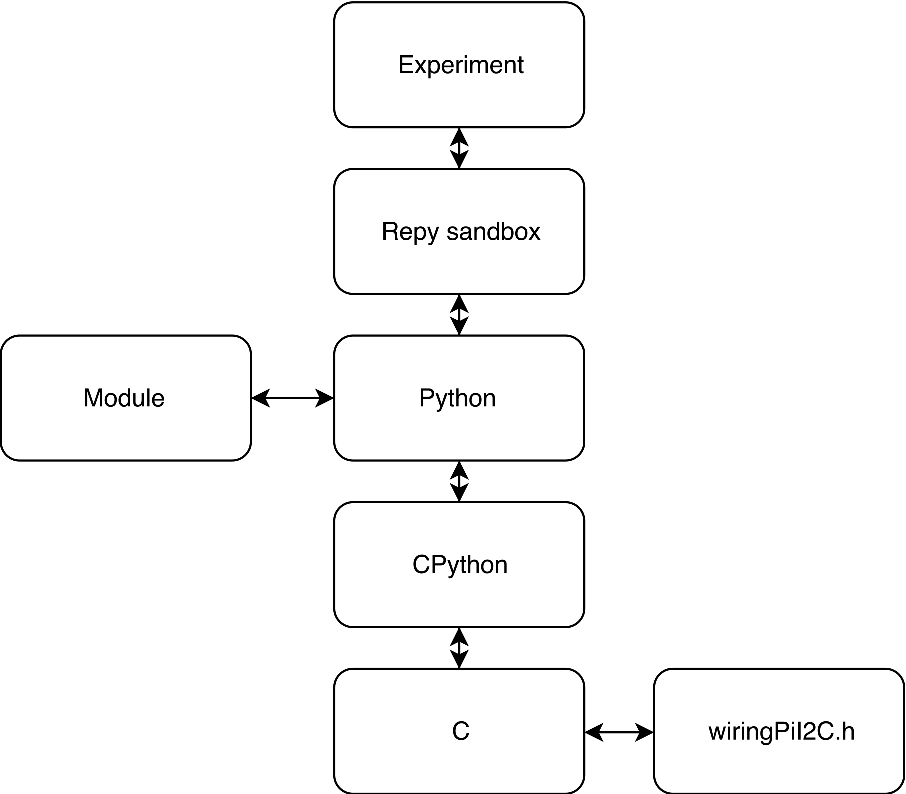
\includegraphics[width=9cm]{CPython_Workflow.pdf}}
	\caption{Path from experiment to C code}
	\label{fig:cPython}
\end{figure}

This work allows the user, in the end, to call the functions through \gls{seash} over the Internet. The message flow when running the \gls{Repy} code provided by the user is illustrated in Figure \ref{fig:cPython}. Here, the experiment calls the \gls{API} in the \gls{Repy} \gls{SB} that runs the Python code. At this point, it was possible to call a Python module that accesses the sensors. Through the CPython \gls{API} the C code is executed and accesses the \gls{I2C} messages through the wiringPi library. The values are then returned to the experiment where it is being processed.

\subsection{Visualization and Website}

A website to visualize the sensor data also is part of this work. The goal of the website was to provide the user with means to visualize his or her data and to have a platform to inform about other information regarding the boxes, as well as developments.

\begin{figure}[ht]
	\makebox[\textwidth][c]{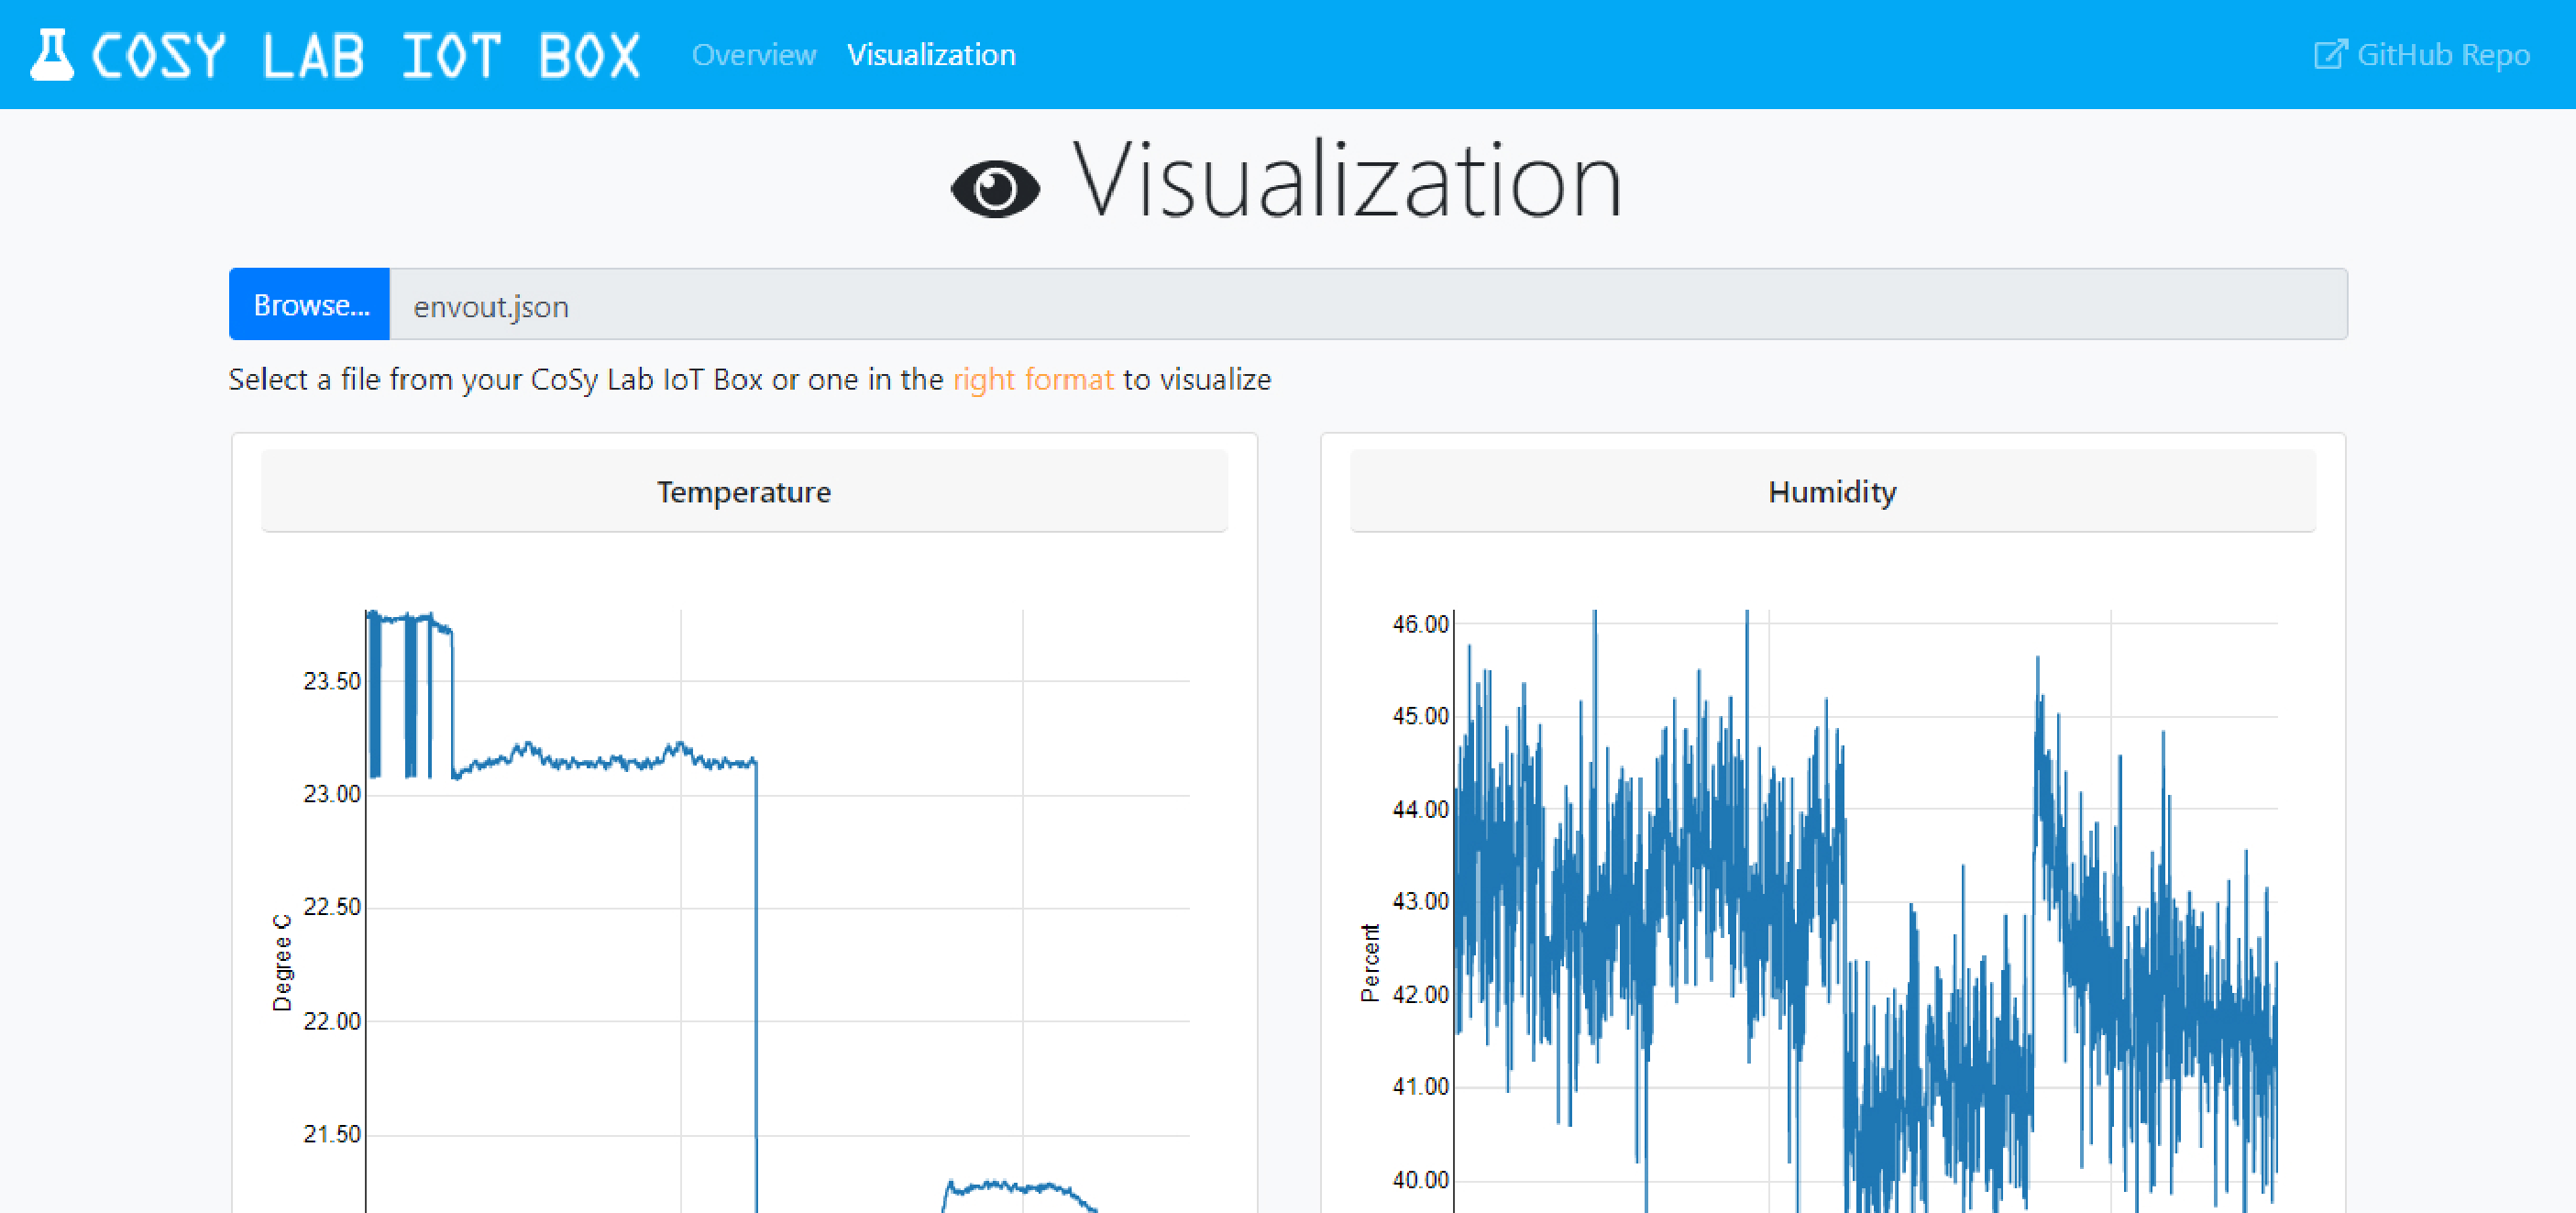
\includegraphics[width=13.5cm]{Website_Mockup.pdf}}
	\caption{Screenshot of the visualization website}
	\label{fig:website}
\end{figure}

The website, that is visible in Figure \ref{fig:website}, uses various libraries and frameworks to offer those features. The front-end was built using Bootstrap\footnote{\url{https://getbootstrap.com/}}, JQuery\footnote{\url{https://jquery.com/}}, and Font Awesome\footnote{\url{https://fontawesome.com/}} (for various kinds of icons). Since Bootstrap is able to optimize a web page for both mobile and desktops, one may view this website on most modern devices at multiple screen resolutions. As a side note the website is just there to showcase the visualization and provide a template for others therefore there is just one web page available as of now.

To plot the charts, the JavaScript library Angular-nvD3\footnote{\url{http://krispo.github.io/angular-nvd3/}} was used. As the name states Angular\footnote{\url{https://angular.io/}}, NVD3\footnote{\url{http://nvd3.org/}} and D3.js\footnote{\url{https://d3js.org/}} are also required to be loaded. They are the back-end of this website and are responsible to build the charts using the data uploaded by the user.

To create a visualization, the user is asked to upload a file in \gls{JSON} format\footnote{\url{https://www.json.org/}}. The function that processes the file searches for a specific key and adds the value and date to the corresponding chart. The available keys used in this project are:

\begin{itemize}
  \setlength\itemsep{0em}
  \item Time
  \item Temperature
  \item Humidity
  \item Pressure
  \item UV
  \item IR
  \item VIS
  \item eCO2
  \item TVOC
\end{itemize}

The collection of key-value pairs is iterated and pushed into the values array of the charts. The charts are refreshed through the \gls{API} from Angular-nvD3 after the last task is finished. The process, after uploading the file, normally takes just a few seconds and depends on the amount of values being inserted.

%%%%%%%%%%%%%%%%%%%%%%%%%%%%%%%%%%%%%%%%%%%%%%%%%%%%%%%%%%%%%%%%%%%%%%%%%%%%%%%%
\section{Evaluation	and	Testing} \label{sec:evaluation}

Many use cases are possible with the \gls{IoT} box and there are a plethora of possibilities to extend it with the available sensors on the market. Therefore, it is not easy to test the box for every eventuality, but some evaluation and testing can be done for the most probable utilization of it.

\subsection{Functional Evaluation}

Working with the box since the first prototype was built, there were some work flows that reoccurred quite often. Based on that a use case scenario was created:

\subsubsection*{\textbf{Use Case Scenario - Collecting Data and Visualizing it}}

\begin{itemize}
  \setlength\itemsep{0em}
  \item A researcher successfully connects over \gls{seash} with his cluster of \gls{IoT} boxes with his personal key
  \item He prepared a \gls{Repy} code that he now uploads to the boxes and starts them
  \item After enough data is collected, the researcher stops the execution of his code and downloads the files that were created during that time period
  \item Fortunately, he saved all those collected values in one JSON file and has now temperature, humidity, pressure, \gls{UV}, \gls{IR}, visible light, \gls{eCO2} and \gls{TVOC} data that he uploads to the web page
  \item The website processes his file and plots graphs for the data that the researcher can analyze
\end{itemize}

Some tests were conducted on the basis of this use case scenario that are shown in Table \ref{tab:funcTest}. Not every function was tested explicitly: some functions are already implemented in Seattle and were not worked on as part of this work, for example up- and downloading files to the boxes.

A majority of the tests worked well. The partial result with the long-term experiment is connected with the other two partial results. As mentioned in Section \ref{sec:airQual}, the air quality sensor does not fully work with the Raspberry Pi. It was just possible to collect data for a shorter period of time than with the others. The other sensors worked properly as we see in Table \ref{tab:funcTest}. Therefore, a long-term experiment is possible if the sensor is not used.

\begin{table}[ht]
\centering
\begin{tabular}{|l|l|}
\hline
\textbf{Test} & \textbf{Result} \\ \hline
Doing a long-term experiment & Partial \\ \hline
Reading temperature & Worked \\ \hline
Reading humidity values & Worked \\ \hline
Reading pressure values & Worked \\ \hline
Reading \gls{UV} values & Worked \\ \hline
Reading \gls{IR} values & Worked \\ \hline
Reading visible light values & Worked \\ \hline
Reading \gls{eCO2} values & Partial \\ \hline
Reading \gls{TVOC} values & Partial \\ \hline
Visualizing collected data & Worked \\ \hline
\end{tabular}
\caption{Tested features of the \gls{IoT} box implementation}
\label{tab:funcTest}
\end{table}

\newpage

\subsection{Experiment Evaluation}

For the experiment the \gls{IoT} box was put on a windowsill during winter in Vienna, on 09.02.2018. Right beneath the window is a heater and the room dimension is 15m\textsuperscript{2} (around 161ft\textsuperscript{2}). According to WetterOnline\footnote{\url{https://www.wetteronline.at/wetterdaten/wien?period=4&month=02&year=2018}}, the outdoor temperature at ''Hohe Warte" was between 0°\gls{C} and 3°\gls{C}. humidity was measured at 74\% and pressure at 1019 \gls{hPa}. The \gls{IoT} box collected data for several hours before the files were downloaded through \gls{seash}. Having the file at hand, it was loaded into the visualization web page to create charts.
\newpage

\begin{figure}[ht]
  \begin{subfigure}[c]{0.5\textwidth}
    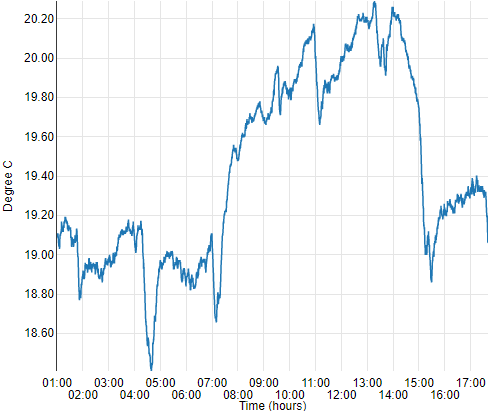
\includegraphics[width=1\textwidth]{expEval/Temp_09-02-2018.PNG}
    \subcaption{Temperature data (in \gls{C})}
    \label{fig:evalTemp}
  \end{subfigure}
  \begin{subfigure}[c]{0.5\textwidth}
    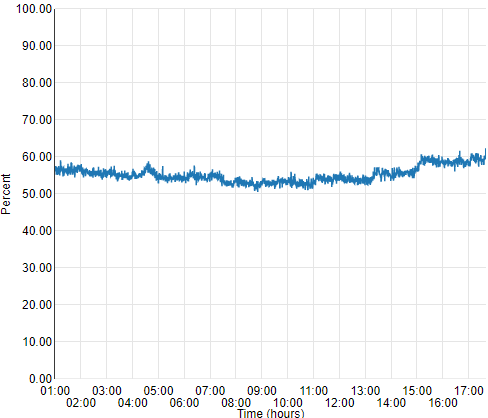
\includegraphics[width=1\textwidth]{expEval/Hum_09-02-2018.PNG}
    \subcaption{Humidity data (in \%)}
    \label{fig:evalHum}
  \end{subfigure}
  \par\medskip
  \begin{subfigure}[c]{\textwidth}
    \centering
    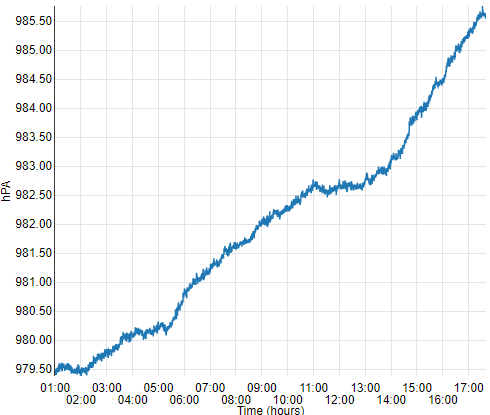
\includegraphics[width=0.5\textwidth]{expEval/Pres_09-02-2018.PNG}
    \subcaption{Pressure data (in \gls{hPa})}
    \label{fig:evalPres}
  \end{subfigure}
  \caption{Data collected by the BME280 sensor}
\end{figure}

Figure \ref{fig:evalTemp} shows the measured temperature. At 7 AM the heating started and the temperature had risen up to its peak at 1:15 PM to 20.30°\gls{C}. At 3 PM, the window was tilted for 30 minutes and the temperature fell 2°\gls{C} before rising again. The lowest point was reached at 4:40 am with a temperature of 18.42°\gls{C}. The mean is 19.43 from all 2000 collected values.

The humidity in Figure \ref{fig:evalHum} did not show significant change. It started at midnight at 56.89\% humidity and in the end just raised by less than 6\% to 62.34\%, its peak. The lowest point was at 7:50 AM with a value of 50.55\% and the mean of 55.24\%. Tilting the window also increased humidity by a small amount. This can be explained by the fact that the window was just tilted and no real exchange of inside and outdoor air happened here.

Comparing the pressure with the information from WetterOnline, it is apparent that it was increasing that day. This also reflects with the values recorded by the box. Starting at 979.39 \gls{hPa}, the numbers grew up to 985.77 \gls{hPa}.

\newpage

\begin{figure}[ht]
\begin{subfigure}[c]{0.5\textwidth}
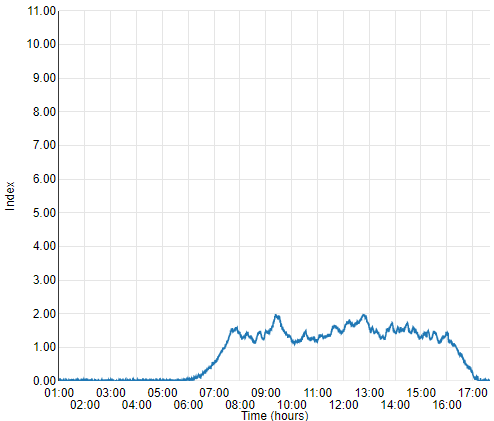
\includegraphics[width=1\textwidth]{expEval/UV_09-02-2018.PNG}
\subcaption{\gls{UV} data (index)}
\label{fig:evalUV}
\end{subfigure}
\begin{subfigure}[c]{0.5\textwidth}
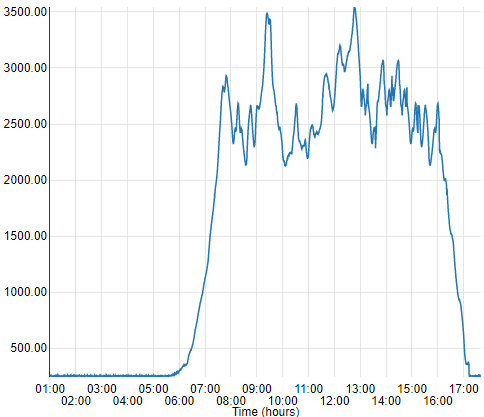
\includegraphics[width=1\textwidth]{expEval/IR_09-02-2018.PNG}
\subcaption{\gls{IR} light data}
\label{fig:evalIR}
\end{subfigure}
\par\medskip
\begin{subfigure}[c]{\textwidth}
\centering
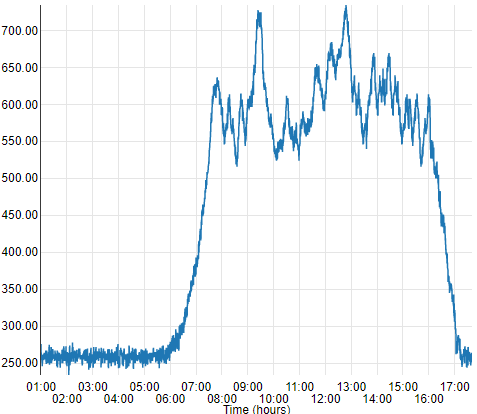
\includegraphics[width=0.5\textwidth]{expEval/VIS_09-02-2018.PNG}
\subcaption{Visible light data}
\label{fig:evalVIS}
\end{subfigure}
\caption{Data collected by the SI1145 sensor}
\end{figure}

On this day, the sunshine was limited. Inspecting Figure \ref{fig:evalIR} and \ref{fig:evalVIS}, we can see that the sunrise was at 7 AM and the sunset happened at 5 PM. The graphs indicate, there are no units to the values because the sensor just measures how much light falls into it. Therefore, it is there for information, but using those two values, it is possible to calculate the \gls{UV} index that is shown in Figure \ref{fig:evalUV}. The World Health Organization categorized the \gls{UV} index into several categories. It is categorized into low (0-2), moderate (3-5), high (6 and 7), very high (8-10) and extreme (11+) \cite{uvDesc}. Hence, the scale of the y-axis in Figure \ref{fig:evalUV}. That day it stayed under two. The value is low enough as to not be harmful to human skin.

\newpage

\begin{figure}[ht]
\begin{subfigure}[c]{0.5\textwidth}
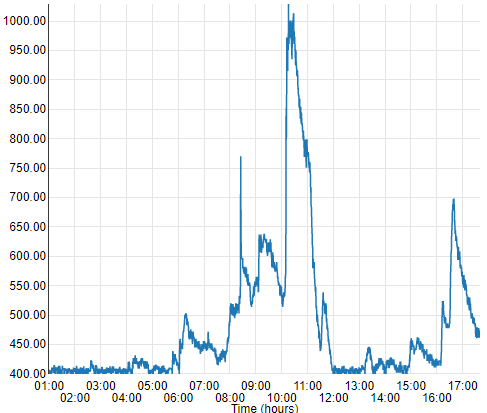
\includegraphics[width=1\textwidth]{expEval/eCO2_09-02-2018.PNG}
\subcaption{\gls{eCO2} data}
\label{fig:evalCO2}
\end{subfigure}
\begin{subfigure}[c]{0.5\textwidth}
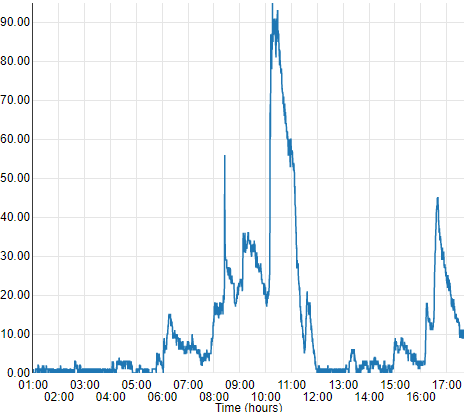
\includegraphics[width=1\textwidth]{expEval/VOC_09-02-2018.PNG}
\subcaption{\gls{TVOC} data}
\label{fig:evalTVOC}
\end{subfigure}
\caption{Data collected by the CCS811 sensor}
\end{figure}

After the 20 minutes burn in that are necessary for the sensor to calibrate correctly, it started to measure some data. The \gls{eCO2} and \gls{TVOC} was at its peak at 10:30 AM with values over 1000 \gls{ppm} and 90 \gls{ppb} respectively. It is shown in Figure \ref{fig:evalCO2} and \ref{fig:evalTVOC} that the two graphs look almost identical. This is because the \gls{eCO2} value is based on the \gls{TVOC} detection. Humans also produce \gls{CO2} and \glspl{VOC} by exhaling it. In this case, analyzing the graphs, every spike means that the room was occupied by one or more persons.


%%%%%%%%%%%%%%%%%%%%%%%%%%%%%%%%%%%%%%%%%%%%%%%%%%%%%%%%%%%%%%%%%%%%%%%%%%%%%%%%
\section{Conclusion} \label{sec:conclusio}

The solution approach presented in this work is combining Seattle with the Raspberry Pi to build \gls{IoT} devices and fetch the sensor data that was collected. After working with the setup for several weeks, it emerged, that the advantages of Seattle made it the suitable candidate as a software base. This advantages were cluster management, code pushing, the \gls{SB} and extendability of the API. The flexibility of the approach made the solution future proof because new sensors can be attached and used with existing ones.

During the implementation, no larger problems were presented. The only negative development was the \gls{TVOC}/\gls{eCO2} sensor that did not properly with the Raspberry Pi. As already described in the functional evaluation, it was still possible to operate with it, but not in the way original intended. That was a small drawback regarding the full functionality of the \gls{IoT} box, but it would be fixable by replacing the sensor with another one.

Additionally, it is possible to configure the \gls{IoT} boxes over the Internet. The boxes need a working connection so the user can upload and start his or her file through \gls{seash}. On the other hand, it also simplifies the process of configuring multiple boxes at once.

\subsection{Future Work}

In the future it would be possible to expand the sensor diversity. There are a lot of different sensors for sale like motion, sound, GPS and plenty more. Even sensors that have not been developed yet and are just future thinking could possibly be paired with a Raspberry Pi which has Seattle installed. 

To conduct some outdoor research, it would be helpful to have support for LoRa and LoRaWAN. LoRaWAN is based on LoRa and is able to store data in a database over a long distance by uploading them through a gateway \cite{lora}. An application server like the visualization website for example could fetch the data and have an up-to-date collection of charts. Using \gls{MQTT}, the data could be available the moment it gets uploaded to the database, if the website subscribes to the broker.

%%%%%%%%%%%%%%%%%%%%%%%%%%%%%%%%%%%%%%%%%%%%%%%%%%%%%%%%%%%%%%%%%%%%%%%%%%%%%%%%
\bibliographystyle{acm}
\bibliography{bibliography/bibliography.bib}

%\section{Appendix}

\end{document}